\stfhIndex{I195}{Bofeng}{波前（wave front）}
\section{\termWaveFront{}与\termBasicPhaseFunction{}}
\label{sec:wave-front-basic-phase-function}

$S=\{\mathrm{pt}\}$ 的情形特别有趣，因为它与拉格朗日子流形
\[
  L=\phi_H^1(o_N)
\]
的\emph{\termWaveFront{}}结构密切相关。\footnote{译者注：原书此处写成 $L=\phi_H(o_N)$，漏掉表示时一像的上标 1；紧随的定义 12.8.1 使用 $\phi_H^1(o_N)$，译文据此补正。}

当 $S=\{\mathrm{pt}\}$ 时，对每个给定的 $H$，$H_0(\{q\})\cong\mathbb Z$ 有一个在符号意义下唯一的生成元；把与它相伴的不变量记为 $\rho(H;\{q\})$。于是，$N$ 上的赋值
\[
  q\longmapsto\rho(H;\{q\})
\]
定义了 $N$ 上的连续函数；这是\cref{prop:spectral-invariant-continuous-in-submanifold}的推论。

\stfhIndex{I040}{Jibenxiangweihanshu}{基本相位函数（basic phase function）}
\begin{definition}
\label{def:basic-phase-function}
把这个函数记为 $f_H:N\to\mathbb R$，亦即
\[
  f_H(q):=\rho(H;\{q\}),
\]
并称之为 $H$ 的\emph{\termBasicPhaseFunction{}}，或 $L=\phi_H^1(o_N)$ 的\termBasicPhaseFunction{}。
\end{definition}

使用“\termPhaseFunction{}”这一名称，是因为在\termFourierIntegralOperator{}的\termMicrolocalAnalysis{}中也会出现类似的函数，并被称为相位函数 (Hor71), (GS77)。可以利用连续性先把 $f_H$ 的定义延拓到任意不必非退化的光滑哈密顿量 $H$，再延拓到第 6.2 节意义下的\termTopologicalHamiltonian{}集合。于是赋值
\[
  H\longmapsto f_H:
  \qquad
  \mathcal H\longrightarrow C^0(N)
\]
分别关于 $\mathcal H$ 的\termHamiltonianTopology{}与 $f_H$ 的 $C^0$ 拓扑定义了连续映射。此外，它还满足
\[
  \operatorname{osc}f_H
  =\max f_H-\min f_H
  \le\lVert H\rVert,
\]
其中 $\lVert H\rVert$ 是\termHoferNorm{}。现在取下确界
\[
  \inf_{H\mapsto L}\lVert H\rVert,
\]
其中 $H\mapsto L$ 表示 $\phi_H^1(o_N)=L$，便得到不等式
\begin{equation}
  \operatorname{osc}f_H
  \le d(o_N,L)
  :=\inf_{H\mapsto L}\lVert H\rVert.
\label{eq:basic-phase-oscillation-hofer-distance}
\end{equation}

\begin{definition}
\label{def:wave-front-exact-lagrangian}
设 $L\subset T^*N$ 是任意正合拉格朗日子流形，且 $h:L\to\mathbb R$ 满足
\[
  i^*\theta=dh.
\]
$L$ 的（与 $h$ 相伴的）\termWaveFront{}，定义为下列映射的像：\footnote{译者注：原书把该映射写成 $L\to\mathbb R\times N$、$x\mapsto(h(x),\pi(x))$，但定理 12.8.3 把函数图置于 $N\times\mathbb R$，图 12.2 也采用 $(q,a)$ 次序。译文依后二者统一交换两个因子。}
\[
  L\longrightarrow N\times\mathbb R,
  \qquad
  x\longmapsto\bigl(\pi(x),h(x)\bigr),
\]
其中 $\pi:T^*N\to N$ 是投影。
\end{definition}

\stfhIndex{I051}{Jiaosan}{焦散（caustics）}
回顾 $h$ 在 $L$ 的每个连通分支上都只差一个加法常数才被确定。一般而言，$h$ 不会在 $N$ 上定义一个单值函数。在 $L$ 的\emph{\termCaustic{}}之外，也就是说，在 $N$ 中由投影
\[
  \pi|_L:L\longrightarrow N
\]
的临界值组成的子集之外，$L$ 可以局部表示为图
\[
  \bigl(q,df(q)\bigr),
\]
其中 $h=f\circ\pi$。然而一般而言，$f$ 不能在整体上定义成可微函数。我们要强调，当 $q$ 变化时，
\[
  \#\bigl(\pi^{-1}(q)\cap L\bigr)
\]
可能发生跳跃。\personEliashberg{} (El87) 把 $L$ 的波前中作为某个连续函数 $f:N\to\mathbb R$ 之图的子集称为\emph{\termSemiSimplePart{}}。一个正合拉格朗日子流形 $L$ 的波前是否一定含有半单部分，并不是显然的问题。

事实表明，谱不变量的构造为这样的半单部分给出了一个典范选择。下面对此作出说明。

\begin{theorem}
\label{thm:basic-phase-selects-wave-front}
令 $G_{f_H}$ 是 $f_H$ 的图。则 $G_{f_H}\subset N\times\mathbb R$ 是 $L$ 的波前的一个\termSemiSimplePart{}。此外，当 $H$ 为\personFloer{}正则时，$f_H$ 在一个零测集之外光滑；对一般的 $H$，$f_H$ 是\personLipschitz{}连续的。
\end{theorem}

\begin{proof}
第一个陈述来自定义 $f_H=\rho(H;\{q\})$，以及 $f_H(q)$ 是 $\mathcal A_H|_{\Omega(\{q\})}$ 的临界值这一事实。因此，
\[
  f_H(q)=\mathcal A_H(z_p^H)
  \qquad\text{对某个}\qquad
  p\in\phi_H^1(o_N)\cap T_q^*N.
\]


当 $H$ 为\personFloer{}正则时，\personLipschitz{}连续性立即来自把\cref{prop:spectral-invariant-continuous-in-submanifold}应用于 $S=\{\mathrm{pt}\}$。对一般的光滑 $H$，只需取一列\personFloer{}正则的光滑哈密顿量 $H_i\to H$，并注意由\cref{prop:spectral-invariant-continuous-in-submanifold}的证明可知，式~\eqref{eq:spectral-invariant-lipschitz-submanifold}中的常数 $C$ 只依赖于 $\operatorname{supp}H$。

最后，由\personFloer{}正则情形的构造，$f_H$ 在一个零测集之外的光滑性是显然的。在这种情形下，$f_H$ 的不可微点集是 $N$ 的一个紧\termStratifiedSubmanifold{}。对一般的 $H$，先注意：若 $H_i\to H$ 于光滑拓扑（事实上 $C^2$ 收敛已经足够），则 $f_{H_i}\to f_H$ 于\termLipschitzTopology{}。于是结论来自\personRademacher{}的经典定理（例如见 (Fe69, Theorem 3.1.6)）：\personLipschitz{}函数几乎处处可微。\footnote{译者注：原书把 Rademacher 的姓氏误拼为 “Radermacher”；译文改用通行拼法。}
\end{proof}

\cref{thm:basic-phase-selects-wave-front}给出了一个简易证明，说明在 $o_N$ 的\termHamiltonianDeformation{}集合上定义的\termHoferDistance{}是非退化的。

\begin{theorem}
\label{thm:hofer-distance-nondegenerate-zero-section-orbit}
设 $d(L_1,L_2)$ 是\personHofer{}距离。则
\[
  d(L_1,L_2)=0
  \quad\Longleftrightarrow\quad
  L_1=L_2.
\]
\end{theorem}

\begin{proof}
先考虑 $L_1=o_N$ 的情形。此时按照定义，
\[
  d(o_N,L_2)=\inf_{H\mapsto L_2}\lVert H\rVert.
\]
现设 $d(o_N,L_2)=0$。则式~\eqref{eq:basic-phase-oscillation-hofer-distance}蕴含
\[
  \operatorname{osc}f_H=0.
\]
也就是说，基本相位函数 $f_H$ 是 $N$ 上的常值函数，因而处处光滑，并且
\[
  df_H(q)=0
\]
对所有 $q\in N$ 成立。因此已经证明
\begin{equation}
  o_N\subset L_2=\phi_H^1(o_N).
\label{eq:zero-section-contained-time-one-image}
\end{equation}
利用 $N$ 的紧性与连通性，不难证明式~\eqref{eq:zero-section-contained-time-one-image}确实蕴含
\[
  o_N=L_2.
\]
这就完成了 $L_1=o_N$ 情形的证明。反方向是显然的。

对一般的对子
\[
  L_1=\phi(o_N),
  \qquad
  L_2=\psi(o_N),
\]
先注意，对任意 $\eta\in\mathcal D_\omega(T^*N)$，都有
\[
  d(L_1,L_2)=d\bigl(\eta(L_1),\eta(L_2)\bigr).
\]
因此，可以把一般情形约化到特殊情形 $L_1=o_N$。
\end{proof}

\begin{figure}[t]
  \centering
  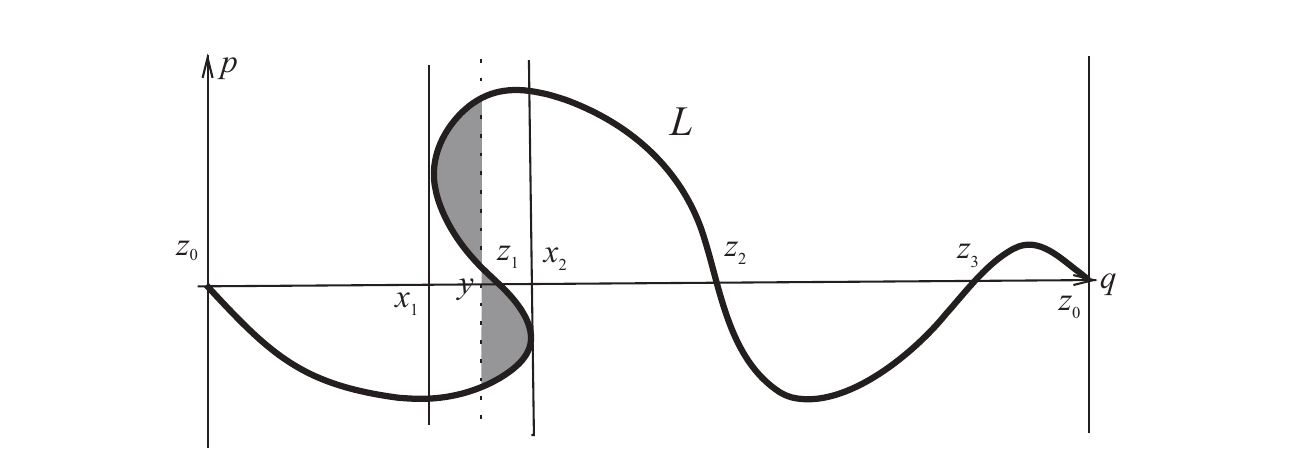
\includegraphics[width=0.9\textwidth]{chapters/ch12-cotangent-floer/figures/ch12-figure-12-1.png}
  \caption{\termMultisectionLagrangian{} $L$。}
  \label{fig:multisection-lagrangian}
\end{figure}

为了说明 $f_H$ 的含义，下面给出 $N=S^1$ 时的一个例子。

\begin{example}
\label{ex:wave-front-circle-multisection}
考虑\cref{fig:multisection-lagrangian}所示的拉格朗日子流形 $L\subset T^*S^1$。这里用 $z_i$ 表示 $L$ 与零截面的交点，用 $x_i$ 表示\termCaustic{}，并用 $y$ 表示图中两个阴影区域面积相等的点。相应的波前不难画成\cref{fig:wave-front-basic-phase}所示。

\begin{figure}[htbp]
  \centering
  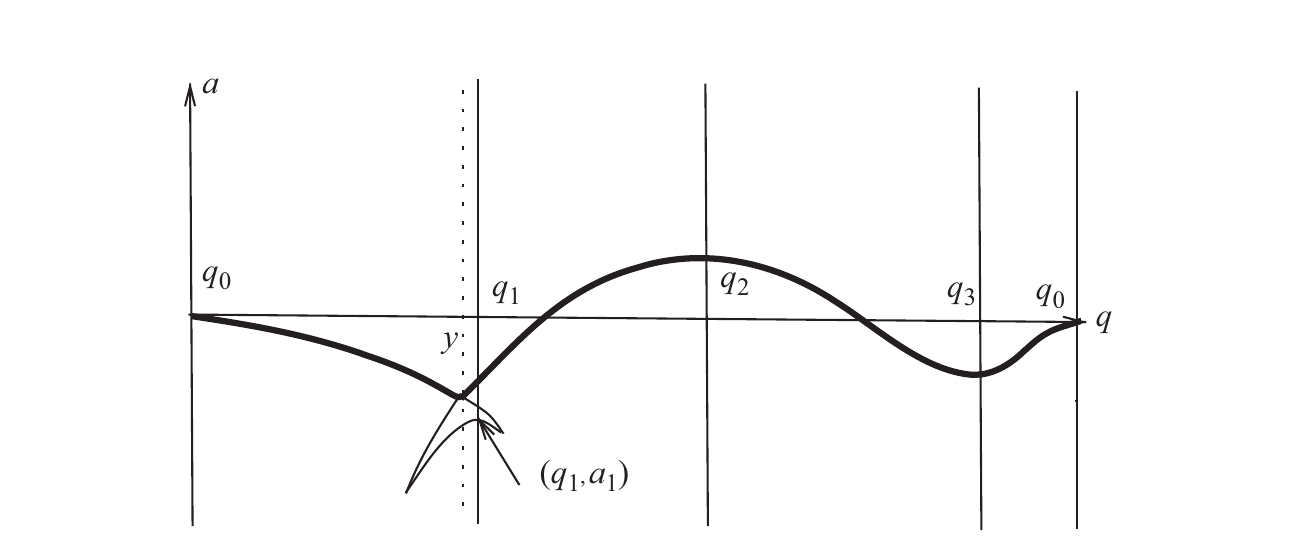
\includegraphics[width=0.88\textwidth]{chapters/ch12-cotangent-floer/figures/ch12-figure-12-2.png}
  \caption{$L$ 的\termWaveFront{}与 $f_H$ 的图。}
  \label{fig:wave-front-basic-phase}
\end{figure}

注意，$z_i$ 对应于作用量泛函的临界点，$x_i$ 对应于波前的\termCuspPoint{}，而 $y$ 对应于波前的两个不同分支相交之点。利用 $H\mapsto L$ 时基本相位函数 $f_H$ 的连续性，不难看出 $f_H$ 的图正是\cref{fig:wave-front-basic-phase}中的粗线。我们还要指出，数值
\[
  \min_{q\in N}f_H(q)
\]
\emph{并不是} $\mathcal A_H$ 的临界值，而是与波前交叉相伴的一个值。\footnote{译者注：原书末句把本节的 $f_H$ 突然写成此前未定义的 $F^H$；译文改回 $f_H$。}
\end{example}
